\documentclass[pdflatex,sn-mathphys-num]{sn-jnl}

\usepackage{graphicx}
\usepackage{multirow}
\usepackage{amsmath,amssymb,amsfonts}
\usepackage{amsthm}
\usepackage[title]{appendix}
\usepackage{xcolor}
\usepackage{textcomp}
\usepackage{manyfoot}
\usepackage{booktabs}
\usepackage{array}
\usepackage{algorithm}
\usepackage{algorithmicx}
\usepackage{algpseudocode}
\usepackage{listings}

\raggedbottom

\AtBeginDocument{\addtolength{\oddsidemargin}{\evensidemargin}\setlength{\oddsidemargin}{0.5\oddsidemargin}\setlength{\evensidemargin}{\oddsidemargin}}
\AtBeginDocument{\let\snOrigThebibliography\thebibliography\renewcommand{\thebibliography}[1]{\snOrigThebibliography{#1}\sloppy\hbadness=10000\relax}}
\makeatletter
\AtBeginDocument{\@ifpackageloaded{hyperref}{\hypersetup{bookmarksdepth=3}}{}}
\makeatother

\begin{document}

\title[Stroke motor imagery decoding with few calibration trials]{Few calibration trials after stroke: pooling patients, session history and online adaptation improve motor imagery decoding}

\author[1]{\fnm{Prayag} \sur{Sharma}}\email{prayag.sharma2024@vitstudent.ac.in}

\author*[2]{\fnm{Ravi} \sur{Tiwari}}\email{ravi.tiwari@vit.ac.in}

\affil[1]{\orgdiv{School of Computer Science and Engineering (SCOPE)}, \orgname{Vellore Institute of Technology}, \orgaddress{\country{India}}}

\affil*[2]{\orgdiv{School of Electronics Engineering (SENSE)}, \orgname{Vellore Institute of Technology}, \orgaddress{\country{India}}}

\abstract{Brain computer interfaces can support motor rehabilitation after stroke, but each patient must first calibrate the decoder, and patients early after a stroke can rarely complete more than a few calibration trials. We propose a decoder that pools the electroencephalography of other patients and of the patient's own earlier sessions in a recentred Riemannian tangent space, splits the motor band into mu, low beta and high beta covariances, and adapts during the session through online recentring, coadaptive updating and online Bayesian model averaging. We evaluated it on three public stroke cohorts, with every confirmatory hypothesis preregistered before the test patients were loaded and tested once. With five calibration pairs of rest and affected hand imagery, pooling other patients raised accuracy on locked test patients from 77.1\% to 81.4\%, more than their own decoder reached with ten pairs, and the gain held on a second cohort of 27 patients, where the band bank added 2.3 points and the patient's earlier sessions 3.2 points. The full decoder raised accuracy on eight locked patients from 77.1\% to 88.7\% in their first session and from 75.9\% to 88.1\% in later sessions, every patient improved, and it exceeded coadaptive recalibration of the patient's own decoder by 3.0 points. Returning patients gained 11.9 points without labels after calibration and 8.4 points with no labels at all, and a gate that uses only calibration data cut the number of patients harmed by transfer from 9 of 16 to 2. The confirmed gains held in audits of trial order, shuffled labels and strictly chronological calibration and on recordings cleaned of artifacts, and a streaming implementation decoded each trial in a median of 12.6 milliseconds. The evidence comes from offline analysis and eight confirmatory patients from one site. At a second hospital, where acute patients imagined moving the left or the right hand, the decoder added 4.4 points over the patient's own decoder but not significantly more than coadaptive recalibration.}

\keywords{Brain computer interface, Electroencephalography, Transfer learning, Riemannian geometry, Neurorehabilitation, Preregistration}

\maketitle

\section{Introduction}\label{sec:intro}

Brain computer interfaces (BCIs) that turn the electroencephalography (EEG) of an attempted movement into feedback can help patients recover arm function after stroke~\cite{mortezaei2026}. The therapy depends on a decoder that recognises each attempt, and motor imagery decoders are trained for each user. Every calibration trial costs effort that a patient early after a stroke can rarely spare, so in practice the decoder has to learn from a handful of trials. Its accuracy is then low, and it varies widely from patient to patient.

A common remedy is to borrow data from elsewhere: from healthy participants, from simulated recordings, from large pretrained models or from other patients (Section~\ref{sec:related}). Two questions about this remedy remain open. The first is which source of borrowed data helps a new stroke patient most when calibration is short. The second comes from the shape of rehabilitation, which runs over many sessions: how far can a returning patient's own earlier recordings replace a fresh calibration? EEG decoding studies are also prone to optimistic evaluation~\cite{brookshire2024}, so an answer to either question needs safeguards against leakage and against selection after the fact.

We therefore built the evaluation before the methods. Test patients were locked away before any method was tuned, a further cohort was kept for validation, and each confirmatory hypothesis was committed to a log under version control before the patients it concerned were loaded, then tested once. On this benchmark we compared the sources of borrowed data, combined those that helped into one decoder that also adapts during the session, and audited the result for leakage. The contributions are the following.
\begin{enumerate}
\item We propose a decoder for calibration with few trials. It pools other patients' recordings and the patient's own earlier sessions in a recentred Riemannian tangent space, uses a bank of mu, low beta and high beta covariances, and adapts during the session through online recentring, coadaptive updating and online Bayesian model averaging (Section~\ref{sec:design}).
\item We assembled a benchmark from three public stroke cohorts and one healthy cohort, harmonised to a common montage and lesion side, with locked test patients, a validation cohort and a timestamped trail of preregistered hypotheses (Section~\ref{sec:setup}).
\item Pooling other patients improved calibration with five trials per class on locked test patients and held on a second cohort, where the band bank and the patient's earlier sessions improved it further. The combined decoder raised accuracy on eight locked patients by about 12 points in their first and later sessions and survived audits of trial order, label permutation, chronological calibration and shared patients (Sections~\ref{sec:res-pooling} to~\ref{sec:res-audit}).
\item A gate that uses only the calibration data decides whether a transferred decoder can be trusted, and a streaming implementation over the Lab Streaming Layer matches the offline results (Section~\ref{sec:res-gate}).
\item We quantify five evaluation pitfalls on these data, each of which produced effects as large as the differences between methods (Section~\ref{sec:res-limits}).
\end{enumerate}

\section{Related work and its limitations}\label{sec:related}

The case for BCI therapy after stroke now rests on syntheses of randomised controlled trials. A meta analysis of 32 such trials with 1187 patients found that noninvasive BCIs improved the Fugl-Meyer score of the upper limb by 3.85 points more than conventional therapy (95\% confidence interval 2.84 to 4.86), and the benefit lasted to follow up~\cite{mortezaei2026}. Another, of 21 trials with 886 patients, found gains in both subacute and chronic patients, and also when the BCI was combined with functional electrical stimulation, a robot or visual feedback~\cite{li2025bci}. Every one of these systems needs a decoder trained on the user, and after stroke the information that the decoder needs may lie in the contralesional rather than the ipsilesional hemisphere~\cite{mansour2022}.

Transfer between users usually begins by aligning their data. Riemannian decoders classify spatial covariance matrices with the geometry of the manifold they live on, either directly by their Riemannian distance to class means or after mapping them to its tangent space~\cite{barachant2012}. Recentring the covariances of every user or session on a reference matrix of their own makes data from different users and sessions comparable, and so makes transfer between them possible~\cite{zanini2018}, and Riemannian Procrustes analysis adds a stretching and a rotation step~\cite{rodrigues2019}. Euclidean alignment whitens each user's trials by their mean covariance in the same spirit, so that any classifier can follow, and it needs no labels from the new user~\cite{he2020}. With deep networks, Euclidean alignment improved the decoding of new subjects by 4.33\% and shortened the convergence of training by more than 70\%~\cite{junqueira2024}, and its correct use and its extensions have since been reviewed~\cite{wu2025ea}. A tutorial on transfer for motor imagery shows that combining alignment with transfer learning in several stages of the pipeline reduces the calibration effort~\cite{wu2022tutorial}.

Deep networks offer a second route. EEGNet is a compact convolutional network for EEG based BCIs that performs well when little training data is available~\cite{lawhern2018}, and deeper convolutional networks trained on raw EEG matched filter bank common spatial patterns and could be visualised~\cite{schirrmeister2017}. After stroke, a deep network pretrained on healthy participants and then adapted to the patients detected motor imagery against rest in 71 patients with a mean accuracy of 71.15\%, and transfer from healthy participants performed as well as transfer from other patients~\cite{nagarajan2024}. On the public cohort of 50 acute patients that we also study~\cite{liu2024}, transferring a reinforcement learning decoder from healthy participants raised the mean success rate in the first epoch only from 49.46\% to 51.82\%; it helped 29 of the 50 patients, and the other 21 showed negative transfer~\cite{via2026}. Within stroke cohorts, a self attention network with partial transfer reached 55.4\% on four classes of motor imagery in 22 patients~\cite{ma2024}, and an ensemble trained across nine chronic patients performed as well as or better than baseline models~\cite{lee2024ensemble}. Foundation models pretrained on large EEG corpora, such as CBraMod, have reached the best published results across many BCI tasks~\cite{wang2025cbramod}. On 30 stroke patients, the LaBraM~\cite{jiang2024labram} and REVE~\cite{elouahidi2025reve} foundation models performed near chance when carried over from healthy participants or when only a new output layer was trained, and low rank adaptation rescued REVE but not LaBraM~\cite{nguyen2026}. Generative augmentation has been used to synthesise a patient's motor imagery features from that patient's own resting EEG, which cut calibration time by 58\% in online tests~\cite{xu2026}.

Adaptation during the session is an older remedy. Coadaptive calibration refits the decoder as cued trials accumulate; it was proposed for novice users and for the estimated 20\% to 25\% of users who cannot control a BCI driven by sensorimotor rhythms~\cite{vidaurre2011}. It needs the label of each trial, which a session driven by cues provides. A returning user's earlier sessions are another source of data: aligned to the few trials of the current session and fused with them, they raised accuracy by over 4\% for 11 stroke patients with only two trials per class, and by about 10\% in sessions that began below 60\%~\cite{giles2022}.

Evaluation practice sets the last constraint. Leakage between training and test data has affected 294 papers in 17 fields that use machine learning, at times with greatly overoptimistic conclusions~\cite{kapoor2023}. In EEG, splitting segments of one participant across training and test sets inflates the accuracy expected on new participants~\cite{brookshire2024}, and theoretical chance levels are too lenient for small test sets, on which purely random signals can reach 70\% or more in two class decoding~\cite{combrisson2015}. Benchmarking frameworks such as the Mother of all BCI Benchmarks (MOABB) make comparisons across datasets trustworthy~\cite{jayaram2018}, and CLEAN-MI harmonises motor imagery datasets from several sources through band filtering, a common channel template, screening of subjects and alignment of their distributions~\cite{liu2025cleanmi}.

These strands leave three gaps. Most of the studies of transfer after stroke cited above borrowed from healthy participants or from generic models; one found healthy and stroke donors equally useful for a deep network~\cite{nagarajan2024}, and we found no study that compared healthy, simulated, pretrained and patient sources head to head on the same stroke patients under short calibration. Rehabilitation runs over many sessions, yet a returning patient's own history has been used only together with labelled trials of the new session~\cite{giles2022}, and not in place of calibration altogether or against other patients' data. Finally, claims in this area are rarely tested on patients locked away in advance under hypotheses fixed beforehand, which is what the evaluation pitfalls above call for.

\section{System design}\label{sec:design}

The decoder and the components around it are described in six subsections: the harmonisation of the recordings (Section~\ref{sec:harmon}), the own and pooled decoders (Section~\ref{sec:decoders}), adaptation during the session (Section~\ref{sec:adapt}), the SafeTransfer gate (Section~\ref{sec:gate-method}), the other sources of borrowed data that the decoder was compared with (Section~\ref{sec:sources}) and the streaming implementation (Section~\ref{sec:stream}). The cohorts, called S1, S3, S4 and H1, are introduced in Section~\ref{sec:cohorts}.

\subsection{Harmonisation}\label{sec:harmon}

All recordings were bandpass filtered between 1 and 40\,Hz, cut from 0.5 to 4.0\,s after the imagery or rest cue, resampled to 128\,Hz (448 samples) and reduced to a motor template of 14 channels (F3, Fz, F4, FC3, FCz, FC4, C3, Cz, C4, CP3, CP4, P3, Pz, P4), rereferenced to their common average. Recordings of patients with left hemiplegia were mirrored across the midline so that every lesion lies in the left hemisphere. In S1 the hand labels were swapped accordingly, so that the right hand always denotes the affected hand, and healthy participants were assigned a virtual lesion in the left hemisphere. Data were loaded with MNE-Python~\cite{gramfort2013} and MOABB~\cite{jayaram2018}. For S1 the original clinical table was used, because a widely mirrored copy of the data lacks the clinical columns. S4 was read from a later release in the Brain Imaging Data Structure (BIDS), whose events mark the onsets of gait imagery and idling, and its paralysed sides came from the participant table of the original release.

\subsection{Own and pooled decoders}\label{sec:decoders}

\paragraph{Own decoder.} For each patient, trials were bandpass filtered between 8 and 30\,Hz, and their spatial covariance matrices $C_i$ were estimated with oracle approximating shrinkage, which suits covariance estimation from few samples~\cite{chen2010}. The covariances were recentred on the Riemannian mean $M$ of the training trials~\cite{zanini2018} and mapped to the tangent space at the identity~\cite{barachant2012},
\begin{equation}
\tilde C_i = M^{-1/2} C_i M^{-1/2}, \qquad s_i = \operatorname{upper}\bigl(\log \tilde C_i\bigr),\label{eq:tangent}
\end{equation}
where $\operatorname{upper}$ stacks the upper triangle of the matrix logarithm, with the entries above the diagonal weighted by $\sqrt{2}$. A logistic regression with an L2 penalty ($C = 1$) classified the vectors $s_i$. The implementation used pyRiemann~\cite{pyriemann}.

\paragraph{Pooled decoder.} Calibration epochs of the target patient were pooled with donor epochs. Each domain, that is every donor and the target's calibration set, was recentred on its own Riemannian mean by Eq.~\eqref{eq:tangent}, which places all of them at the identity~\cite{zanini2018}. One logistic regression was then fitted on all the tangent vectors, with the donor epochs weighted so that all donors together carry the same total weight as the calibration epochs. Donors were the other development patients, healthy participants or simulated stroke data; in S4 they were the other 26 patients.

\paragraph{Band bank.} The pooled decoder with a band bank estimates the covariances separately in the mu (8 to 13\,Hz), low beta (13 to 20\,Hz) and high beta (20 to 30\,Hz) bands. Each band is recentred per domain, and the three tangent vectors are placed side by side before the logistic regression. The theta band, which the best development variant also contained, was left out because eye movements separate rest from imagery there (Section~\ref{sec:res-sweep}).

\paragraph{Earlier sessions.} For a later session of a patient, after treatment or at follow up, the patient's own earlier sessions served as donors. Each session was recentred on its own mean, and all of them together were weighted like the calibration epochs. In the variant without new labels, a decoder was trained on the earlier sessions alone, and the later session was recentred on its calibration epochs without using their labels.

\paragraph{Window ensemble.} For S1, sixteen own decoders were fitted on the training trials, one for each combination of four windows (0.5 to 4, 0.5 to 2.5 and 2 to 4\,s after the imagery cue, and 4 to 6\,s, the period after imagery) and four bands (mu from 8 to 13\,Hz, beta from 13 to 30\,Hz, the range from 8 to 30\,Hz and a filter bank of all three). Their predicted probabilities were averaged. We call this window ensemble ens16.

\subsection{Adaptation during the session}\label{sec:adapt}

The combined decoder builds pooled decoders from four parts and averages several of them online.
\begin{itemize}
\item \textbf{Features:} the band bank, on the template of 14 channels or on a strip of 28 central channels (the F, FC, C and CP rows and P3, Pz and P4, without frontal pole, temporal or occipital channels).
\item \textbf{Donor groups:} the other patients' recordings of the same session and, in later sessions, the patient's own earlier sessions. Each group together weighs as much as the patient's labelled trials.
\item \textbf{Online recentring:} before each test trial, the patient's reference mean $M$ in Eq.~\eqref{eq:tangent} is updated with the calibration trials and every earlier test trial. This needs no labels.
\item \textbf{Coadaptive updating:} before each test trial, the logistic regression is refitted on the calibration trials and every earlier test trial, each with its cue label~\cite{vidaurre2011}. A training session driven by cues knows these labels.
\end{itemize}
Two variants use no labels during the session. The first fits the logistic regression on the labelled calibration trials and the donors, and refits it only as the recentring changes. The second, for returning patients, trains the logistic regression on the earlier sessions alone, so that only the recentring adapts and no label of the current session is used.

When the classes alternate, as in S3 and S1, an update after every trial lets the decoder learn the label of the trial just before, which also tells it where the next trial lies in the alternation. The audited decoders therefore update only at the start of each pair of trials, so that every update sees one trial of each class (Section~\ref{sec:res-audit}).

The full system averages the predicted probabilities $p_{j,i}$ of several decoders $j$ for test trial $i$. Each decoder is weighted by its likelihood on the test trials decoded so far, whose cue labels $y_t$ arrive after each decision:
\begin{equation}
\hat p_i = \frac{\sum_j w_{j,i}\, p_{j,i}}{\sum_j w_{j,i}}, \qquad \log w_{j,i} = \sum_{t < i} \log\bigl(y_t\, p_{j,t} + (1 - y_t)(1 - p_{j,t})\bigr).\label{eq:bma}
\end{equation}
This is Bayesian model averaging with a uniform prior over the decoders. With updates in pairs, the sum in Eq.~\eqref{eq:bma} runs over complete earlier pairs only. The members were fixed before the first development run: static and coadaptive band bank decoders on 14 and 28 channels, a variant with an empirical Bayes prior on the decoder weights and, in later sessions, the stacks with earlier sessions. That gives six members in the first session and ten in later sessions.

\subsection{SafeTransfer gate}\label{sec:gate-method}

For each patient, every candidate decoder (the own decoder first, then the transferred decoder and the average of the two) was scored by cross validation on the calibration pairs alone, leaving out one pair at a time. The gate selects the best candidate, with ties going to the own decoder, but only if its calibration accuracy beats chance by the exact binomial test at $\alpha = 0.05$ with Bonferroni correction over the candidates. Otherwise it abstains, and the system reports that more calibration is needed instead of giving feedback that may mislead.

\subsection{Other sources of borrowed data}\label{sec:sources}

\paragraph{Deep transfer.} EEGNet~\cite{lawhern2018} was trained with Euclidean alignment~\cite{he2020}, random crops of 2\,s and the AdamW optimiser, pretrained for 60 epochs on donor data and finetuned for 40 epochs on the target's calibration data, with the implementation from braindecode~\cite{schirrmeister2017}. Euclidean alignment needs the inverse square root of the mean covariance. Data referenced to the common average have a null direction, so directions with variance below $10^{-6}$ of the largest were dropped rather than inverted (Section~\ref{sec:res-limits}).

\paragraph{Foundation model.} CBraMod~\cite{wang2025cbramod}, pretrained by masked reconstruction on a very large EEG corpus, was used frozen. Epochs were resampled to 200\,Hz and scaled to units of 100\,\textmu V, as the model expects. The embeddings of patches of 1\,s were averaged and classified by shrinkage linear discriminant analysis trained on the calibration epochs.

\paragraph{LesionSim.} LesionSim turns healthy imagery epochs into epochs that resemble stroke by editing band envelopes while keeping the phase. A band component $b(t)$ of a channel is split by the Hilbert transform into amplitude $A(t)$ and phase $\varphi(t)$, the amplitude is edited into $A'(t)$, and
\begin{equation}
b'(t) = A'(t)\cos\varphi(t)\label{eq:lesionsim}
\end{equation}
replaces $b(t)$. With the edit switched off, the output equals the input exactly, which unit tests enforce. The rest amplitude $A_0$ of each channel is taken from the participant's own rest epochs. Three operators define the edited amplitude $A'(t)$ in Eq.~\eqref{eq:lesionsim}. They followed a preliminary comparison of S1 with H1 on development data, which found greater variability of beta activity at C3 between trials in stroke ($p = 0.005$ after Holm correction) and a trend toward reduced laterality. They also followed reports of more variable and more diffuse modulation in stroke EEG~\cite{via2026} and of activity moving to the contralesional hemisphere with severity~\cite{mansour2022}.
\begin{itemize}
\item \textbf{O1, weaker desynchronisation on the lesioned side:} $A' = A_0 + \alpha\,(A - A_0)$ on ipsilesional channels in the mu band, where $\alpha = 1$ leaves the data unchanged.
\item \textbf{O2, contralesional shift:} a share $\beta$ of each ipsilesional channel's relative desynchronisation is added to its mirror channel.
\item \textbf{O4b, variability:} each trial's ipsilesional desynchronisation is scaled by a lognormal gain whose logarithm has standard deviation $s$, in the mu and beta bands.
\end{itemize}
After editing, epochs were rereferenced to the common average, like real data. LesionSim was evaluated in three modes. In population mode, settings were drawn for each participant ($\alpha \sim U(0.6, 1)$, $\beta \sim U(0.2, 0.8)$, $s = 0.5$). In matched mode, $\alpha$ and $\beta$ were estimated from the target patient's calibration epochs, as the ratio of the patient's to the healthy mean relative mu desynchronisation on FC3, C3 and CP3, and as its excess on FC4, C4 and CP4. In learned mode, 27 settings ($\alpha \in \{1, 0.6, 0.2\}$, $\beta \in \{0, 0.4, 0.8\}$, $s \in \{0, 0.5, 1\}$) were scored, and one was chosen honestly with four folds over patients, chosen on 12 and scored on 4.

\subsection{Streaming implementation}\label{sec:stream}

The decoders were packaged for streaming use. A playback process publishes a recording's raw EEG of 64 channels and its cue markers as Lab Streaming Layer (LSL) streams~\cite{kothe2025}, paced in real time, as an amplifier and a stimulus program would. A receiver applies a causal filter between 1 and 40\,Hz, cuts each trial's window as soon as it has arrived, harmonises it, calibrates on the first five pairs of rest and imagery trials and then decodes every later epoch with the own and the pooled decoder. The decoders are the same code as in the offline evaluation, and unit tests check that they give identical outputs.

\section{Experimental setup}\label{sec:setup}

Six subsections describe how the decoders were evaluated: the cohorts (Section~\ref{sec:cohorts}), the protocols and locked test sets (Section~\ref{sec:protocols}), preregistration and statistics (Section~\ref{sec:stats}), the development, confirmation and audits of the combined decoder (Section~\ref{sec:combo-setup}), the secondary analyses (Section~\ref{sec:secondary}) and how each run is organised, with the full experimental grid (Section~\ref{sec:repro}).

\subsection{Cohorts}\label{sec:cohorts}

Table~\ref{tab:cohorts} summarises the four cohorts: the source and task of each, and how many of its patients served for development and how many were locked away for testing.
\begin{itemize}
\item \textbf{S1}~\cite{liu2024}: 50 acute stroke patients, 1 to 30 days after onset, who imagined grasping with the left or the right hand in 40 alternating trials (2\,s instruction, 4\,s imagery, 2\,s break), recorded with 29 EEG and 2 electrooculography (EOG) channels at 500\,Hz.
\item \textbf{S3}~\cite{wang2026}: 24 chronic stroke patients, 3 to 14 months after onset, recorded with 59 EEG channels at 250\,Hz at three time points. Each run interleaves rest, imagery of the affected hand and imagery of a supernumerary sixth finger. Task B pairs every epoch of affected hand imagery with the rest epoch immediately before it, which gives 40 pairs per patient at the first time point.
\item \textbf{S4}~\cite{liu2025gait}: 27 stroke patients, 1 to 12 months after onset (18 with right and 9 with left hemiplegia), who imagined walking or stayed idle in 10 plus 10 trials per run, in random order, recorded with 60 EEG channels before treatment, after treatment and at follow up. It served first as the validation cohort and, once its confirmatory tests were spent, as development data for the combined decoder.
\item \textbf{H1}, the PhysioNet motor movement and imagery database~\cite{schalk2004,goldberger2000}: 109 healthy participants.
\end{itemize}
S3 and S4 were recorded at the same institution with the same amplifier family. Ages, sexes and paralysed sides suggest that some patients may appear in both cohorts, although no S3 data enter any S4 analysis; Section~\ref{sec:res-audit} tests whether this matters. A further cohort, HEFMI-ICH~\cite{shi2025}, with 20 patients after intracerebral haemorrhage and 17 healthy controls recorded with EEG and functional near infrared spectroscopy, was screened but excluded from decoding. Its channel order and labels were verified against the stored metadata and against the topography of alpha with eyes closed, yet the power of its healthy controls in the motor band varied by only about 3\% across the whole trial, which leaves too little desynchronisation related to imagery to decode.

\begin{table}[!htbp]
\caption{Cohorts. Dev, development patients, used to build and compare methods; Locked, test patients held out and used once for each preregistered hypothesis. S4 served first as the validation cohort and then as development data for the combined decoder.}\label{tab:cohorts}
\footnotesize
\begin{tabular}{@{}l>{\raggedright\arraybackslash}p{0.30\textwidth}>{\raggedright\arraybackslash}p{0.36\textwidth}rr@{}}
\toprule
 & Cohort & Task used here & Dev & Locked\\
\midrule
S1 & Liu et al.~\cite{liu2024}, acute stroke, Beijing & Task A: imagery of the left versus the right hand & 34\footnotemark[1] & 15\\
S3 & Wang et al.~\cite{wang2026}, chronic stroke, Tianjin & Task B: imagery of the affected hand versus rest & 16 & 8\\
S4 & Liu et al.~\cite{liu2025gait}, stroke, Tianjin & Gait imagery versus idling, three sessions & none & 27\footnotemark[2]\\
H1 & PhysioNet~\cite{schalk2004,goldberger2000}, healthy & Imagery of the left or the right hand, and rest & \multicolumn{2}{r}{109 donors}\\
\botrule
\end{tabular}
\footnotetext[1]{Of 35. One patient failed a quality rule that uses no labels (median correlation between neighbouring channels below 0.3, observed 0.08) and was excluded before any decoding.}
\footnotetext[2]{Validation cohort, all patients. The later sessions of four patients are missing from the public release, and one follow up session had fewer than the preregistered minimum of 20 trials per class.}
\end{table}

\subsection{Protocols and locked test sets}\label{sec:protocols}

Before any method was tuned on a cohort, a stratified random subset of its patients was locked away. In S1, 15 of 50 patients were locked, stratified by paralysed side and by a score on the National Institutes of Health Stroke Scale (NIHSS) above the median; in S3, 8 of 24, stratified by paralysed side and by time since stroke above the median. Locked patients were loaded only to test a hypothesis that had been written down and committed beforehand (Table~\ref{tab:prereg}). S4 served as a validation cohort: its four hypotheses were committed while its download was still running, amended before any of its recordings was decoded, and each was tested once on all patients.

Two protocols were used within patients. Blocked cross validation, used for S1 development, splits a patient's 40 trials into four contiguous blocks of ten and tests each block with a model trained on the other three, so that slow drifts cannot leak between training and test trials. Chronological calibration, used for S1 screening and for all of S3 and S4, calibrates on the first $k$ trials of each class in recording order, or on the first $k$ pairs of rest and imagery trials, and tests on all remaining trials, as a clinical session would. Here $k$, the number of calibration trials per class, was 5 or 10. Every reference statistic, filter, recentring matrix and model was fitted on training or calibration trials only.

\subsection{Preregistration and statistics}\label{sec:stats}

Hypotheses, the frozen pipeline and the test statistic were committed to the project's results log before the locked patients were loaded, and the commits are listed in Tables~\ref{tab:prereg} and~\ref{tab:prereg-combo}. Each confirmatory analysis was run once, and its outcome was reported whatever it was. Comparisons are paired across patients: Wilcoxon signed rank tests on the accuracy of each patient, with zero differences dropped, Holm correction within each family of comparisons~\cite{holm1979}, and bootstrap 95\% confidence intervals (CIs) of the mean. Accuracy differences were rounded to $10^{-9}$ before ranking, so that differences that are equal in exact arithmetic are treated as ties (Section~\ref{sec:res-limits}).

The four hypotheses for S4 (H-R1 to H-R4) were tested in a fixed sequence: the pooling hypothesis first at $\alpha = 0.05$ and, only if it held, the other three with Holm correction. The six hypotheses about the combined decoder (H-C1 to H-C6) and the three for the second hospital (H-E1 to H-E3) were each tested in a fixed sequence at $\alpha = 0.05$. Noninferiority used a margin of 2 points, the preregistered threshold for harm, and a patient counts as harmed when a method scores at least 2 points below the patient's own decoder. Significance for a single patient uses the exact one sided binomial test~\cite{combrisson2015}; with 39 test trials, an accuracy of at least 66.7\% is required.

\subsection{Development, confirmation and audits of the combined decoder}\label{sec:combo-setup}

In two declared rounds, 27 decoders were compared on the 16 S3 development patients and on S4. Because the confirmatory tests of S4 were spent, it counted as development data. Selection was made without hindsight, by leaving one patient out at a time and across cohorts, and this phase is exploratory. A third declared round added seven decoders and a larger model average. Six hypotheses about the frozen decoders (H-C1 to H-C6) were then committed and tested once on the eight S3 locked patients in all their sessions, with the 16 development patients as donors. Before that run, no combination decoder had been applied to these patients. A declared sensitivity analysis applied the same tests to the dataset authors' recordings of the same patients, cleaned with independent component analysis (ICA).

A declared audit then checked the combined decoder for leakage and overfitting in five ways.
\begin{enumerate}
\item \textbf{Trial order:} the online decoders and the averaging weights were also evaluated with updates in pairs (Section~\ref{sec:adapt}).
\item \textbf{Label permutation:} every patient's labels were shuffled within each session, donors included, and every decoder had to fall to chance.
\item \textbf{Chronological calibration in S4:} every trial up to the one that completes $k$ per class calibrates, so that no test trial precedes a calibration trial.
\item \textbf{Causality:} unit tests check that each online decision uses only earlier trials.
\item \textbf{Shared patients:} patients possibly shared by S3 and S4 were identified from demographics and covariance fingerprints, and the tests were also run without them.
\end{enumerate}
Finally, three further hypotheses (H-E1 to H-E3) were committed and tested once on all 49 usable S1 patients. They used the frozen decoders on 14 channels, because S1 lacks the strip of 28, and updates in pairs, because the hands of S1 alternate too.

\subsection{Secondary analyses}\label{sec:secondary}

\paragraph{Sweep.} On the 16 S3 development patients, the pooled decoder was varied one design choice at a time and in combinations: 14, 28 or all 59 channels; the window from 0.5 to 4.0\,s or from 0.5 to 5.5\,s; single bands, band banks and an ensemble of nine members; donor weights from 0.5 to 8 times the calibration; regularisation; the 8 nearest or best fitting donors; stretching of each domain to unit dispersion~\cite{rodrigues2019}; a linear support vector machine (SVM); synthetic calibration epochs mixed in; no labels; and online adaptation. The sweep also covered the same patients' sessions after treatment, and the gain of picking the best variant was estimated without hindsight by leaving one patient out at a time.

\paragraph{Artifact controls.} Own and pooled decoders were also trained on channel groups that should carry little motor signal, each rereferenced to its own average: frontal channels from 1 to 8\,Hz for eye movements, occipital or posterior channels from 8 to 30\,Hz for visual cortex, and temporal channels for muscle. The raw EOG channels of S3 could not be regressed out, because in most runs they were flat or far outside the physiological range. The decoders were therefore also evaluated on the cleaned release published by the dataset authors (43 channels, average reference, ICA). Whether the confirmed S3 result survives this cleaning was checked once on the locked test patients. This sensitivity analysis was declared in the log before it was run, and it could not add a confirmed result.

\paragraph{Neurophysiology.} For S3 (all 24 patients, described with fixed methods) and the healthy cohort, the event related desynchronisation (ERD) of each channel was computed as $(\bar A_{\mathrm{MI}} - \bar A_{\mathrm{rest}}) / \bar A_{\mathrm{rest}}$, where $\bar A_{\mathrm{MI}}$ and $\bar A_{\mathrm{rest}}$ are the mean Hilbert envelopes during motor imagery and rest, in the mu and beta bands. To explain why some donors help, each patient's direction separating imagery from rest in the recentred tangent space (the difference of class means, scaled to unit length) was compared by cosine similarity with the pooled direction of the healthy donors and with that of the other patients. The reliability of that direction between odd and even pairs gives the ceiling. Finally, the own decoder's accuracy in blocked cross validation was compared across the three S3 time points.

\paragraph{Analyses of S1.} The baseline methods published with S1 were evaluated on its raw data with the analysis code released with the dataset~\cite{liu2024}. An audit that used no labels counted faulty channels and rhythm peaks, and further decoders were compared with the own decoder under blocked cross validation.

\subsection{Runs and experimental grid}\label{sec:repro}

A single run takes one cohort from the public files to a table of accuracies. The loader reads the recordings, harmonises them (Section~\ref{sec:harmon}) and caches the spatial covariance matrices of every band and channel set. For every patient and session, the run splits the trials into calibration and test sets, fits each decoder on the calibration trials and the donors, decodes the test trials in recording order and writes one row per patient, session and $k$ with the accuracy of every decoder. Each finished patient and session is saved at once, so that an interrupted run resumes where it stopped, and a separate script computes every statistic and figure from the saved rows.

The grid of the combined decoder, read from the saved result files, was as follows.
\begin{itemize}
\item \textbf{Development:} in S3, 16 patients in 45 sessions (16 before treatment, 16 after treatment and 13 at follow up); in S4, 27 patients in 72 sessions (27, 23 and 22). With two calibration sizes, $k = 5$ and $k = 10$, a run gives 90 rows for S3 and 144 for S4. The first two rounds compared 27 decoders, and the third added seven decoders and a larger model average.
\item \textbf{Confirmation:} 8 locked S3 patients in 22 sessions (8, 8 and 6), on raw and on cleaned recordings, with 44 rows each.
\item \textbf{External test:} 49 S1 patients, 98 rows.
\item \textbf{Audits:} the first two rounds evaluated with updates in pairs (S3 development and locked patients, raw and cleaned), with shuffled labels (S3 development and S4) and with chronological calibration (S4).
\end{itemize}
Each secondary experiment settles one question, and its result appears where indicated.
\begin{itemize}
\item \textbf{Sources of borrowed data on S3} (deep transfer, a frozen foundation model, healthy and simulated donors, other patients): which source helps when calibration is short? Sections~\ref{sec:res-pooling} and~\ref{sec:res-limits}.
\item \textbf{Sweep of 39 decoders in the first session and 40 in the second:} which design choices improve the pooled decoder? Section~\ref{sec:res-sweep}.
\item \textbf{Artifact controls and the cleaned release:} do signals other than motor activity drive the decoding? Section~\ref{sec:res-sweep}.
\item \textbf{Neurophysiology of S3 and H1:} why are other patients better donors than healthy participants? Section~\ref{sec:res-neuro}.
\item \textbf{SafeTransfer on S3 development patients:} can calibration data alone prevent harmful transfer? Section~\ref{sec:res-gate}.
\item \textbf{Streaming playback of the eight locked S3 patients:} does the online pipeline match the offline results? Section~\ref{sec:res-gate}.
\item \textbf{LesionSim in three modes:} can simulated stroke data stand in for real patients? Section~\ref{sec:res-limits}.
\item \textbf{Decoders and published baselines on S1:} how decodable is imagery of the left versus the right hand in acute stroke? Section~\ref{sec:res-limits}.
\end{itemize}

\section{Results and discussion}\label{sec:results}

Eight subsections follow. Sections~\ref{sec:res-pooling} to~\ref{sec:res-s4} report the confirmed effect of pooling, the design choices behind the band bank and the validation on S4. Sections~\ref{sec:res-combo} and~\ref{sec:res-audit} report the combined decoder, its audits and its test at a second hospital. Section~\ref{sec:res-neuro} explains why other patients make good donors, Section~\ref{sec:res-gate} covers the safety gate and streaming operation, and Section~\ref{sec:res-limits} reports what did not help, the evaluation pitfalls and the limitations of the study. Tables~\ref{tab:prereg} and~\ref{tab:prereg-combo} collect every preregistered test with its outcome.

\begin{table}[!htbp]
\caption{Preregistered confirmatory tests of pooling, of its validation on S4 and of two decoders for S1. Each hypothesis was committed to the results log under version control (commit shown) before the patients were loaded, and was run once. Tests are one sided Wilcoxon signed rank tests over patients; the S4 tests ran in a fixed sequence, with H-R2 to H-R4 Holm corrected. $n$, patients.}\label{tab:prereg}
\footnotesize
\setlength{\tabcolsep}{3pt}
\begin{tabular}{@{}>{\raggedright\arraybackslash}p{0.31\textwidth}c>{\raggedright\arraybackslash}p{0.46\textwidth}>{\raggedright\arraybackslash}p{0.13\textwidth}@{}}
\toprule
Hypothesis (commit) & $n$ & Result & Verdict\\
\midrule
S3: pooling other patients beats the own decoder at $k = 5$ pairs (\texttt{d916f30}, 24 Oct 2026) & 8 & 77.1\% $\rightarrow$ 81.4\% (+4.3 points); 7 helped, 1 harmed; $p = 0.047$\footnotemark[1]. Secondary, $k = 10$: +2.1 points, $p = 0.17$ & Confirmed\\
\addlinespace
S4, H-R1: the same pooling on a second cohort (\texttt{d0800e8}, 31 Oct 2026) & 27 & 69.1\% $\rightarrow$ 70.8\% (+1.6, 95\% CI +0.2 to +3.1); 14 helped, 6 harmed; $p = 0.019$ & Confirmed\\
\addlinespace
S4, H-R2: a band bank of mu, low beta and high beta beats the pooled decoder (\texttt{0d9b750}) & 27 & 70.8\% $\rightarrow$ 73.1\% (+2.3, CI +0.5 to +4.1); 17 helped, 6 harmed; Holm $p = 0.021$ & Confirmed\\
\addlinespace
S4, H-R3: the patient's earlier sessions beat the own decoder in later sessions (\texttt{0d9b750}) & 23 & 67.4\% $\rightarrow$ 70.7\% (+3.2, CI +1.5 to +5.1); 15 helped, 4 harmed; Holm $p = 0.0045$ & Confirmed\\
\addlinespace
S4, H-R4: without new labels, the earlier sessions' decoder is not 2 points or more worse than five labelled calibration pairs (\texttt{0d9b750}) & 23 & 69.7\% versus 67.4\% (+2.3, CI $-1.2$ to +5.7); Holm $p = 0.021$ & Confirmed noninferior\\
\addlinespace
S1: the window ensemble beats the base decoder (\texttt{e1556cc}, 21 Oct 2026) & 15 & 54.4\% $\rightarrow$ 58.0\% (+3.6); 7 helped, 3 harmed, 5 tied; $p = 0.083$ & Not confirmed\\
\addlinespace
S1: patients passed by a calibration screen on the first 20 trials decode later trials better than those it abstains on (\texttt{d916f30}) & 15 & 1 patient passed (78.9\%) versus 14 abstained (53.9\%), specified in advance as not evaluable with fewer than 2 per group. Secondary: Spearman $\rho = 0.37$, $p = 0.088$ & Not evaluable\\
\botrule
\end{tabular}
\footnotetext[1]{Computed with accuracy differences rounded to $10^{-9}$, so that equal differences are treated as ties. Without rounding, floating point noise separates them and the test gives 0.035 (Section~\ref{sec:res-limits}).}
\end{table}

\begin{table}[!htbp]
\caption{Preregistered confirmatory tests of the combined decoder, each run once in a fixed sequence at $\alpha = 0.05$ with one sided Wilcoxon signed rank tests over patients. H-C1 to H-C6 concern the eight S3 locked patients, where later is each patient's mean over the sessions after treatment and at follow up, and the smallest attainable $p$ is 0.0039. H-E1 to H-E3 concern all 49 usable S1 patients, which earlier analyses had used, so all of them were tested together. $n$, patients.}\label{tab:prereg-combo}
\footnotesize
\setlength{\tabcolsep}{3pt}
\begin{tabular}{@{}>{\raggedright\arraybackslash}p{0.31\textwidth}c>{\raggedright\arraybackslash}p{0.46\textwidth}>{\raggedright\arraybackslash}p{0.13\textwidth}@{}}
\toprule
Hypothesis (commit) & $n$ & Result & Verdict\\
\midrule
S3, H-C1: the combined decoder with online model averaging beats the own decoder, first session (\texttt{ec5cd82}, 1 Nov 2026) & 8 & 77.1\% $\rightarrow$ 88.7\% (+11.6); 8 helped, 0 harmed; $p = 0.0039$. Updates in pairs\footnotemark[1]: 89.1\% (+12.0), $p = 0.0039$ & Confirmed\\
\addlinespace
S3, H-C2: the same, later sessions & 8 & 75.9\% $\rightarrow$ 88.1\% (+12.2); 8 helped, 0 harmed; $p = 0.0039$. In pairs: 87.9\% (+12.0), $p = 0.0039$ & Confirmed\\
\addlinespace
S3, H-C3: the combined decoder beats coadaptive recalibration of the own decoder, first session & 8 & 83.5\% $\rightarrow$ 88.7\% (+5.2); 7 helped, 1 harmed; $p = 0.020$. In pairs: 86.0\% $\rightarrow$ 89.1\% (+3.0); 7 helped, 1 harmed; $p = 0.047$ & Confirmed\\
\addlinespace
S3, H-C4: earlier sessions, other patients and online recentring, without labels after calibration, beat the own decoder, later sessions & 8 & 75.9\% $\rightarrow$ 87.7\% (+11.9); 8 helped, 0 harmed; $p = 0.0039$. In pairs: 87.4\% (+11.5), $p = 0.0039$ & Confirmed\\
\addlinespace
S3, H-C5: the earlier sessions' decoder with online recentring and no labels at all beats the own decoder with five labelled pairs, later sessions & 8 & 75.9\% $\rightarrow$ 84.2\% (+8.4); 8 helped, 0 harmed; $p = 0.0039$. In pairs: 83.8\% (+7.9), $p = 0.0039$ & Confirmed\\
\addlinespace
S3, H-C6: other patients, band bank and online recentring, without labels after calibration, beat the own decoder, first session & 8 & 77.1\% $\rightarrow$ 85.8\% (+8.7); 7 helped, 1 harmed; $p = 0.0078$. In pairs: unchanged & Confirmed\\
\addlinespace
S1, H-E1: the combined decoder on 14 channels, with updates in pairs, beats the own decoder at a second hospital, five trials per hand (\texttt{484842c}, 1 Nov 2026) & 49 & 52.5\% $\rightarrow$ 56.9\% (+4.4); 31 helped, 14 harmed; $p = 0.0027$ & Confirmed\\
\addlinespace
S1, H-E2: the same beats coadaptive recalibration of the own decoder & 49 & 56.2\% $\rightarrow$ 56.9\% (+0.7); 24 helped, 17 harmed; $p = 0.17$ & Not confirmed\\
\addlinespace
S1, H-E3: other patients, band bank and online recentring, without labels after calibration, beat the own decoder & 49 & 52.5\% $\rightarrow$ 57.1\% (+4.6); descriptive $p = 0.0009$ & Not tested, sequence stopped\\
\botrule
\end{tabular}
\footnotetext[1]{Audit (Section~\ref{sec:res-audit}): the online decoders and averaging weights were updated only between pairs of rest and imagery trials, so that no update carries a trial's position in the alternating sequence of S3. The preregistered runs updated after every trial.}
\end{table}

\subsection{Pooling other patients shortens calibration}\label{sec:res-pooling}

Task B of S3 is far easier than Task A of S1: the own decoder reached 81.7\% with five calibration pairs and 84.7\% with ten. Pooling the other development patients' recordings was the only strategy that improved on it. With five pairs it reached 84.0\%, a median gain of 1.4 points ($p = 0.003$, or 0.012 after Holm correction); 11 of 16 patients were helped, and none was harmed by 2 points or more. With ten pairs it reached 86.1\% (+0.8 points, $p = 0.20$). The preregistered test on the eight locked patients confirmed the result with five pairs (Table~\ref{tab:prereg}): accuracy rose from 77.1\% to 81.4\%, with 7 patients helped, 1 harmed and all 8 above chance afterwards. Figure~\ref{fig:pooling}a,b shows these gains patient by patient with five pairs, for the development and for the locked patients. Each line is a patient, red where accuracy fell, which matters because a mean gain can hide patients who were harmed. Figure~\ref{fig:pooling}c gives the mean accuracy of both decoders in both groups with five and with ten pairs, with bootstrap 95\% CIs. Pooled decoding with five calibration pairs (81.4\%) matched the own decoder with ten (79.5\%), which halves the calibration needed.

\begin{figure}[!htbp]
\centering
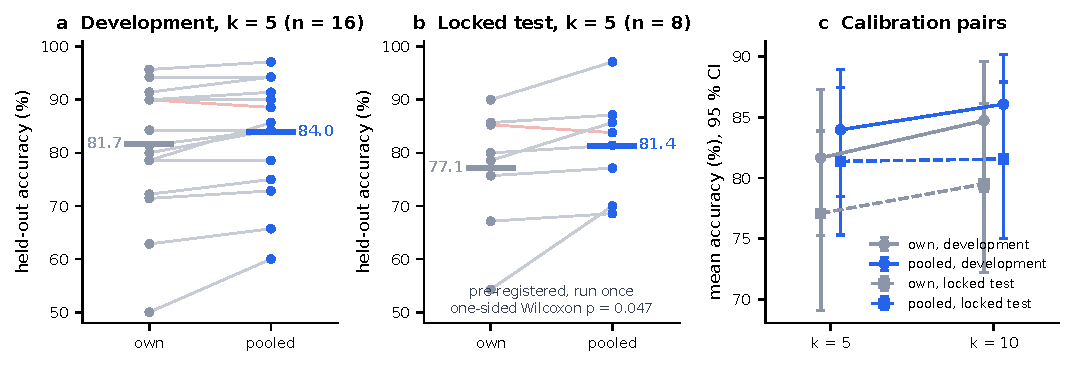
\includegraphics[width=\textwidth]{figures/fig1_pooling.pdf}
\caption{Pooling other patients (S3): (a) development and (b) locked patients; (c) means.}\label{fig:pooling}
\end{figure}

Figure~\ref{fig:strategies} places pooling among every source of borrowed data that we tried, on the same patients, with five calibration pairs in Figure~\ref{fig:strategies}a and ten in Figure~\ref{fig:strategies}b, so that its gain can be judged against the alternatives. Each point is the mean over the 16 development patients with its bootstrap 95\% CI, the dotted line marks the own decoder, and EEGNet and CBraMod are the deep network and the foundation model of Section~\ref{sec:sources}. Other patients' recordings were the only source that improved on the own decoder at either calibration size. Healthy data, LesionSim and the frozen foundation model stayed at or below it; Section~\ref{sec:res-limits} gives their numbers.

\begin{figure}[!htbp]
\centering
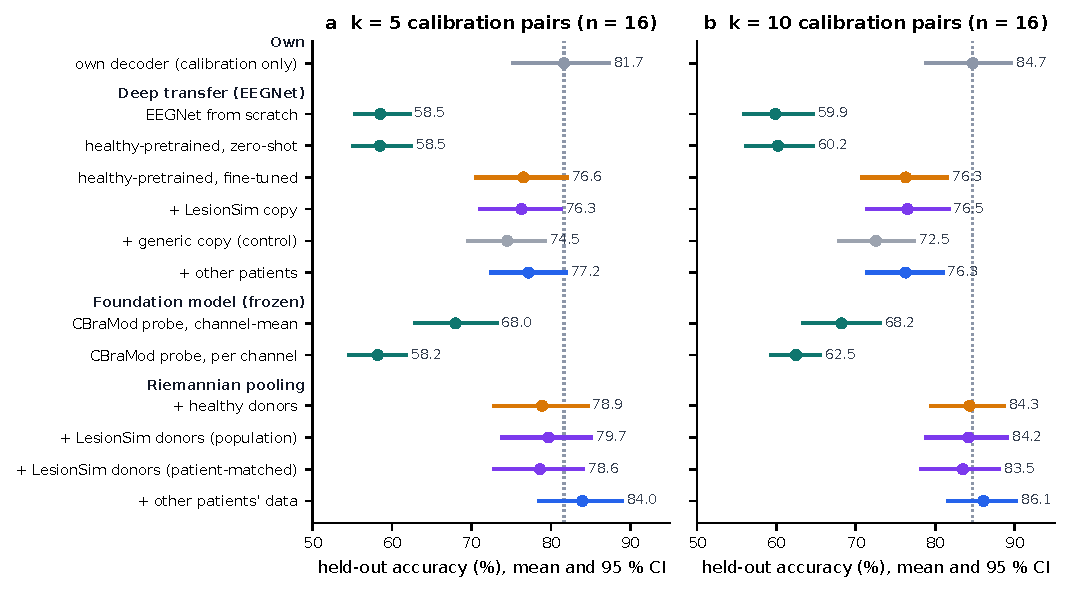
\includegraphics[width=\textwidth]{figures/fig2_transfer_strategies.pdf}
\caption{Sources of borrowed data (S3): (a) five and (b) ten calibration pairs.}\label{fig:strategies}
\end{figure}

\subsection{Design choices and signals outside the motor cortex}\label{sec:res-sweep}

The sweep compared 39 decoders in the first session and 40 in the second, the own and pooled decoders included. Figure~\ref{fig:robustness}a shows the gain of each variant over the pooled decoder for the 16 development patients in both sessions, with five calibration pairs, which separates choices that help consistently from those that help once. No variant with fixed calibration survived Holm correction over the 31 comparisons of the first session.
\begin{itemize}
\item \textbf{Splitting the band helped most consistently.} A bank of theta, mu, low beta and high beta covariances added 3.0 and 3.7 points over the pooled decoder in the two sessions ($p = 0.004$ in the second session; 13 helped, 2 harmed). Mu alone was worse by 4.7 points ($p = 0.045$ after Holm correction).
\item \textbf{More channels helped somewhat.} Using 28 or 59 channels added between 1.2 and 2.7 points, and up to 4.8 with a band bank, mostly in the second session. Part of this came from channels outside the motor strip, as shown below.
\item \textbf{Other choices did not help.} A longer window, donor weighting, choosing the nearest or best fitting donors, stretching, an SVM, an ensemble of nine and synthetic calibration epochs changed the mean by between $-1.9$ and $+0.8$ points; stretching cost the most.
\item \textbf{Honest selection gained little.} Picking the best variant without hindsight gained 1.8 points in the first session ($p = 0.22$) and 3.0 in the second ($p = 0.020$).
\item \textbf{The protocol mattered most.} The only gain that survived Holm correction came from refitting the decoder after every trial with its cue label: coadaptive recalibration reached 88.6\% against 84.0\% ($p = 0.012$ after Holm correction). Once labels kept arriving, pooling added nothing, and the own decoder recalibrated in the same way reached 88.5\%.
\end{itemize}
The band bank without its theta band was carried forward as hypothesis H-R2 for S4, for the following reason.

Channels far from the motor cortex also separated imagery from rest in S3. On the development patients, the own decoder with five pairs reached 77.3\% on frontal channels from 1 to 8\,Hz, where eye movements and blinks dominate, 74.3\% on occipital channels from 8 to 30\,Hz, 66.1\% on temporal channels and only 60.3\% on frontal channels from 8 to 30\,Hz. The strict motor strip (the FC, C and CP rows) reached 81.1\%, close to the template of 14 channels (81.7\%). Figure~\ref{fig:robustness}b compares these channel groups in the raw recordings and in the dataset authors' release cleaned with ICA: after cleaning, the eye control fell to 55.2\%, while motor decoding stayed between 83.6\% and 84.1\%. Cleaning raised the own decoder enough that the pooled decoder with a single band no longer beat it (84.0\% versus 83.6\%), but the pooled decoder with the band bank still did (86.0\% versus 84.1\%, $p = 0.020$; 9 helped, 1 harmed).

The declared sensitivity analysis on the cleaned recordings of the eight locked patients gave the same picture (Figure~\ref{fig:robustness}c). Pooling with a single band gained 1.6 points over the own decoder ($p = 0.29$), and pooling with the band bank gained 3.5 points ($p = 0.031$; 4.8 points with ten pairs, $p = 0.031$). Posterior channels still separated the classes after cleaning (72.2\%), so part of what a decoder of imagery versus rest detects in this paradigm is probably visual or attentional engagement rather than motor imagery alone. We therefore recommend the version with the band bank, and we suggest that studies of imagery versus rest report controls on channels outside the motor cortex.

\begin{figure}[!htbp]
\centering
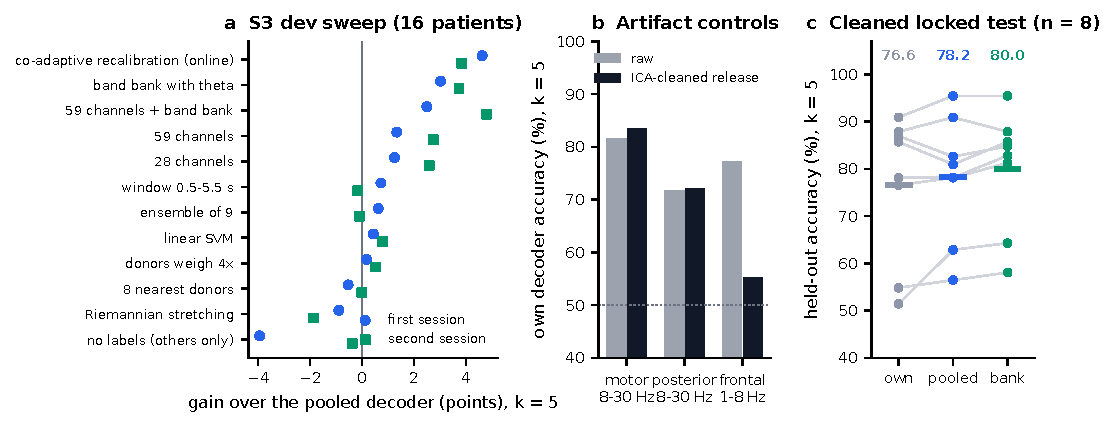
\includegraphics[width=\textwidth]{figures/fig8_robustness.pdf}
\caption{Design choices and artifact controls (S3): (a) decoder variants, (b) channel groups, (c) cleaned locked patients.}\label{fig:robustness}
\end{figure}

\subsection{A second cohort, the band bank and returning patients}\label{sec:res-s4}

All four preregistered hypotheses held on S4, each tested once with five calibration trials per class (Table~\ref{tab:prereg}). Figure~\ref{fig:s4} shows each of them patient by patient, with one line per patient, red where accuracy fell.
\begin{itemize}
\item \textbf{Pooling held on the second cohort.} Pooling the other 26 patients raised accuracy with five calibration trials per class from 69.1\% to 70.8\% ($p = 0.019$; 14 helped, 6 harmed; Figure~\ref{fig:s4}a). The gain was smaller than on S3, at a lower level of accuracy, for a different limb and with randomised rather than paired trials.
\item \textbf{The band bank added more.} It reached 73.1\%, which is 2.3 points over the pooled decoder ($p = 0.021$ after Holm correction) and 4.0 over the patient's own decoder (Figure~\ref{fig:s4}b).
\item \textbf{Earlier sessions helped.} In the sessions after treatment and at follow up, the patient's own earlier sessions raised accuracy by 3.2 points on average ($p = 0.0045$ after Holm correction; Figure~\ref{fig:s4}c, averaged over both later sessions for each patient): by 5.4 points at follow up (17 helped, 2 harmed) and by 1.5 after treatment. The S3 development patients showed the same pattern, with 4.7 points at follow up (9 helped, 1 harmed; $p = 0.031$ after Holm correction).
\item \textbf{No new labels were needed.} The earlier sessions' decoder, without labels from the later session, reached 69.7\% against 67.4\% for the own decoder with five labelled pairs, which is noninferior at the margin of 2 points ($p = 0.021$ after Holm correction; Figure~\ref{fig:s4}d). On the S3 development patients at follow up it reached 84.5\% against 77.9\%.
\end{itemize}
Descriptively, coadaptive recalibration also gave the largest single gain, 75.2\% for the own decoder (+6.1 points). A decoder from the other patients alone, without labels, reached 68.5\% ($-0.7$ points), and a band bank on 59 channels 77.9\%. Channels outside the motor cortex carried less information than in S3: frontal channels from 1 to 8\,Hz reached 64.9\% and occipital channels 63.7\%.

\begin{figure}[!htbp]
\centering
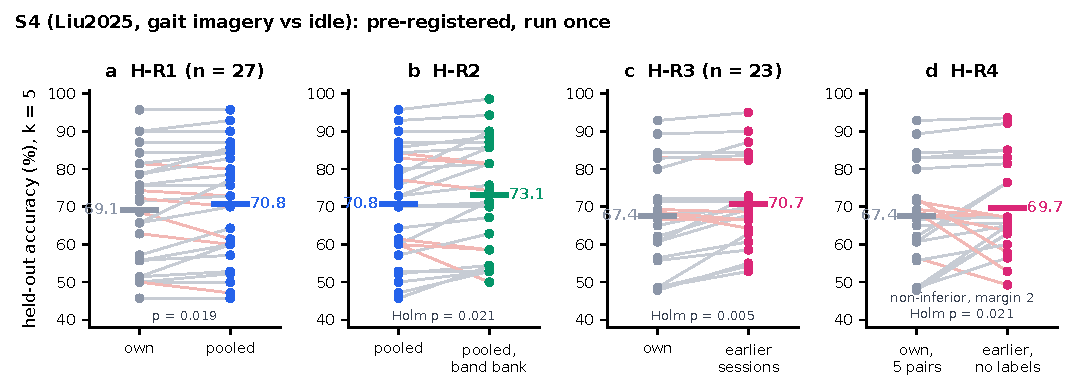
\includegraphics[width=\textwidth]{figures/fig7_s4.pdf}
\caption{Preregistered validation on S4: (a) H-R1, (b) H-R2, (c) H-R3 and (d) H-R4.}\label{fig:s4}
\end{figure}

\subsection{The combined decoder}\label{sec:res-combo}

\paragraph{Development.} The gains added up. Figure~\ref{fig:combo}a,b traces the mean accuracy of the development patients of S3, raw and cleaned with ICA, and of S4 as each part joins the own decoder, in the first session and for returning patients, which shows how much of the total each part contributes. The parts join in the order listed below, and those in the grey area need the cue label of every trial during the session. With five calibration pairs, in both development cohorts:
\begin{itemize}
\item \textbf{First session.} Other patients and the band bank lifted the own decoder by 4 to 5 points, and online recentring, which needs no labels, added 1 to 2 points. Coadaptive updating with the cue labels and model averaging brought the total to 9.3 points on S3 (81.7\% $\rightarrow$ 91.0\%) and 11.2 points on S4 (69.1\% $\rightarrow$ 80.3\%; 26 of 27 patients helped).
\item \textbf{Returning patients.} The earlier sessions, the other patients and the band bank on 28 channels together gained 8.0 points on both cohorts without labels after calibration. With online recentring they gained 8.8 and 9.8 points, and with coadaptive updating and model averaging 10.3 and 11.6 points.
\item \textbf{Beyond coadaptive recalibration.} Model averaging beat coadaptive recalibration of the patient's own decoder, the established technique, in every cohort and setting: by 2.6 and 4.0 points on S3 with updates in pairs, and by 5.1 and 6.1 points on S4, in the first and later sessions.
\item \textbf{Choices transferred across cohorts.} The best decoder picked on S3 scored 11.2 points (first session) and 11.6 points (returning patients) above the own decoder on S4, and the best decoders picked on S4 scored 9.3 and 10.3 points above it on S3.
\item \textbf{Artifacts.} On the cleaned development recordings, the coadaptive stacks kept most of their gain: 6.2 points in the first session, and 7.4 and 8.6 points in later sessions. So did the stack for returning patients without labels after calibration, at 7.3 points, while the static decoders without labels kept about half.
\end{itemize}

\paragraph{Confirmation on the locked patients.} All six preregistered hypotheses held (Table~\ref{tab:prereg-combo}), and Figure~\ref{fig:combo}c,d shows every locked patient's accuracy with the own decoder and with the full stack, in the first session and in later sessions, where each patient's two later sessions are averaged.
\begin{itemize}
\item With coadaptive updating and model averaging, accuracy rose from 77.1\% to 88.7\% in the first session and from 75.9\% to 88.1\% in later sessions, and every patient improved in both settings.
\item In the first session the stack beat coadaptive recalibration of the own decoder by 5.2 points (7 of 8 patients); the audit in Section~\ref{sec:res-audit} lowered this margin to 3.0 points.
\item Without labels after calibration, returning patients reached 87.7\% (+11.9 points, 8 of 8) and first session patients 85.8\% (+8.7, 7 of 8).
\item With no labels at all in the later session, the earlier sessions' decoder with online recentring reached 84.2\%, which is 8.4 points above the own decoder with five labelled pairs (8 of 8).
\item With ten calibration pairs, the full stack gained 7.7 points in the first session and 12.5 in later sessions, and every patient improved.
\end{itemize}
The declared sensitivity analysis on the cleaned recordings of the same patients gave the same verdicts for all six hypotheses (one sided $p$ between 0.004 and 0.039). The full stack gained 10.6 points in the first session (7 of 8 patients) and 12.8 in later sessions (8 of 8), and it beat coadaptive recalibration of the own decoder by 4.9 points. The stacks without labels gained 12.4 points (returning patients, no labels after calibration), 9.5 (no labels at all) and 6.9 (first session).

\begin{figure}[!htbp]
\centering
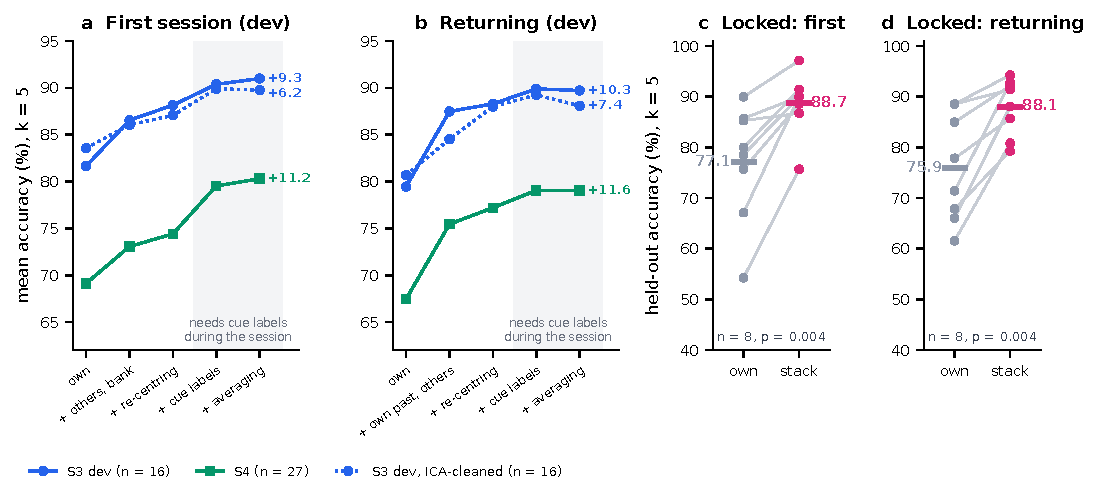
\includegraphics[width=\textwidth]{figures/fig9_combination.pdf}
\caption{The combined decoder: (a, b) development patients and (c, d) S3 locked patients.}\label{fig:combo}
\end{figure}

For clinical use, two of these results matter more than the headline. Without any labels after calibration, the stack still gained about 12 points for returning patients, so a session paced by the patient, which cannot rely on cues, would benefit too. With no labels at all in a returning session, the patient's earlier sessions and online recentring beat a fresh calibration of five pairs by 8 points, so from the second session on, labelled calibration can be skipped.

\subsection{Audits and a second hospital}\label{sec:res-audit}

The declared audit for leakage and overfitting left every verdict standing.
\begin{itemize}
\item \textbf{Trial order.} The trials of S3 alternate between rest and imagery, so an update after every trial can carry a trial's position in the sequence. With updates only between pairs of rest and imagery trials, the stack gained 12.0 points in the first session and 12.0 in later sessions (both $p = 0.0039$), and all six hypotheses held on raw and on cleaned recordings (Table~\ref{tab:prereg-combo}). Updating after every trial had handicapped coadaptive recalibration of the own decoder, which just before each imagery trial had learned the label of the paired rest trial. Updated in pairs, it reached 86.0\% instead of 83.5\%. The honest margin of the stack over it is therefore 3.0 points (7 of 8 patients, $p = 0.047$), and 2.6 points on the cleaned recordings ($p = 0.016$).
\item \textbf{Shuffled labels.} With every patient's labels shuffled within each session, donors included, all 27 decoders scored between 47\% and 52\% on the S3 development patients and on S4. Model averaging scored 48.5\% and 49.1\%, against 91.0\% and 80.3\% with the true labels. The smallest $p$ value against 50\%, 0.007, came from the highest of 27 decoders (pooling with a single band in the later sessions of S4, 52.3\%) in one of 216 checks over decoders and settings, which chance explains.
\item \textbf{Chronological calibration.} With five trials per class, the first trials of each class calibrate, so in the randomised order of S4 some test trials precede the last calibration trial. With strictly chronological calibration, model averaging scored 80.6\% and 79.1\% in the first and later sessions of S4 (80.3\% and 79.1\% before), 13.6 and 11.9 points above the own decoder (27 of 27 and 22 of 23 patients helped). Only the own decoder lost accuracy, because its calibration set became imbalanced between the classes.
\item \textbf{Shared patients.} Two locked S3 patients may also appear in S4: each matches an S4 patient in age, sex and lesion side, and covariance fingerprints could not settle the question. Without them, all six hypotheses still held ($p = 0.016$ each, 6 of 6 patients helped).
\item \textbf{Causality.} Unit tests confirm that each online decision depends only on earlier trials and labels and, with updates in pairs, only on complete earlier pairs.
\end{itemize}

Applied unchanged to all 49 usable S1 patients, with a different hospital, amplifier, stage (acute) and task (imagery of the affected versus the unaffected hand), the stack with updates in pairs beat the own decoder with five calibration trials per hand. Accuracy rose from 52.5\% to 56.9\% (+4.4 points; 31 helped, 14 harmed; $p = 0.0027$; H-E1). It did not beat coadaptive recalibration of the own decoder, which reached 56.2\% on its own (+0.7 points, $p = 0.17$; H-E2), and this stopped the fixed sequence. The stack without labels after calibration scored 57.1\% (+4.6 points, descriptive $p = 0.0009$; H-E3, not tested). With ten trials per hand the gain shrank to 1.6 points ($p = 0.14$). On this weak signal of the left versus the right hand, the stack helped with very short calibration, and coadaptive recalibration alone delivered most of that help.

\subsection{Why other patients make better donors}\label{sec:res-neuro}

Relative to rest, the 24 chronic patients desynchronised more than the 109 healthy participants almost everywhere, and Figure~\ref{fig:neuro}a maps this difference over the template channels, averaged over participants, with the lesion on the left after harmonisation and, for healthy participants, the left hemisphere contralateral to the imagined right hand. Stroke desynchronisation was stronger, wider and shifted, not weaker.
\begin{itemize}
\item In the mu band, patients reached between $-17\%$ and $-25\%$, against between $-6\%$ and $-17\%$ for healthy participants. The difference was significant at 11 of 14 channels (Mann--Whitney tests after Holm correction); the exceptions were C3, Cz and CP3, where the healthy focus lies.
\item In the beta band, the difference was significant at all 14 channels.
\item Laterality reversed. Healthy desynchronisation was stronger over the hemisphere contralateral to the imagined hand, whereas the patients' was stronger over the contralesional hemisphere: the laterality index was $+0.11$ versus $-0.10$ in mu and $+0.13$ versus $-0.17$ in beta, both with $p < 0.001$.
\end{itemize}
The shift agrees with the contralesional recruitment reported in more impaired patients~\cite{mansour2022}, and it is what operator O2 imitates. The stronger ipsilesional desynchronisation contradicts the premise of operator O1. Recording system and paradigm also differ between the cohorts and may contribute to the overall difference in magnitude.

The patients' decision directions agreed with each other. In the recentred tangent space, each patient's direction separating imagery from rest was closer to the pooled direction of the other patients than to that of the healthy donors (median cosine 0.87 versus 0.78; Wilcoxon $p = 0.0002$; closer for 22 of 24 patients; Figure~\ref{fig:neuro}b). The median reliability between two halves of a patient's own data, 0.92 and drawn as the dotted line, is the ceiling, so the other patients' direction comes close to what more of the patient's own data would give. This is the mechanism behind the pooling result. Recentring removes each patient's average covariance, and what transfers is the direction. Other patients supply a direction almost as good as more of the patient's own data, healthy donors supply a biased one, and LesionSim did not correct the bias.

Decodability was stable across the study period. The own decoder's accuracy in blocked cross validation did not change significantly between the three S3 time points (Figure~\ref{fig:neuro}c): it was 87.8\% before treatment ($n = 24$), 85.8\% after treatment ($n = 24$) and 85.6\% at follow up ($n = 19$). The change from before to after treatment was $-2.0$ points ($p = 0.18$), and the change from before treatment to follow up $-2.1$ points ($p = 0.11$ after Holm adjustment). Mu desynchronisation over C3 and C4 was also unchanged ($p = 0.46$ and 0.44). A decoder calibrated in one session therefore faces a stable target in this cohort, and the pooled donors need not be stratified by time point. The same argument explains why a patient's own earlier sessions transfer so well: the direction is the patient's own, and it did not drift. The practical conclusion is to pool real patient data across hospitals rather than synthesise it, to keep each patient's recordings from session to session, and to share stroke recordings in harmonised form.

\begin{figure}[!htbp]
\centering
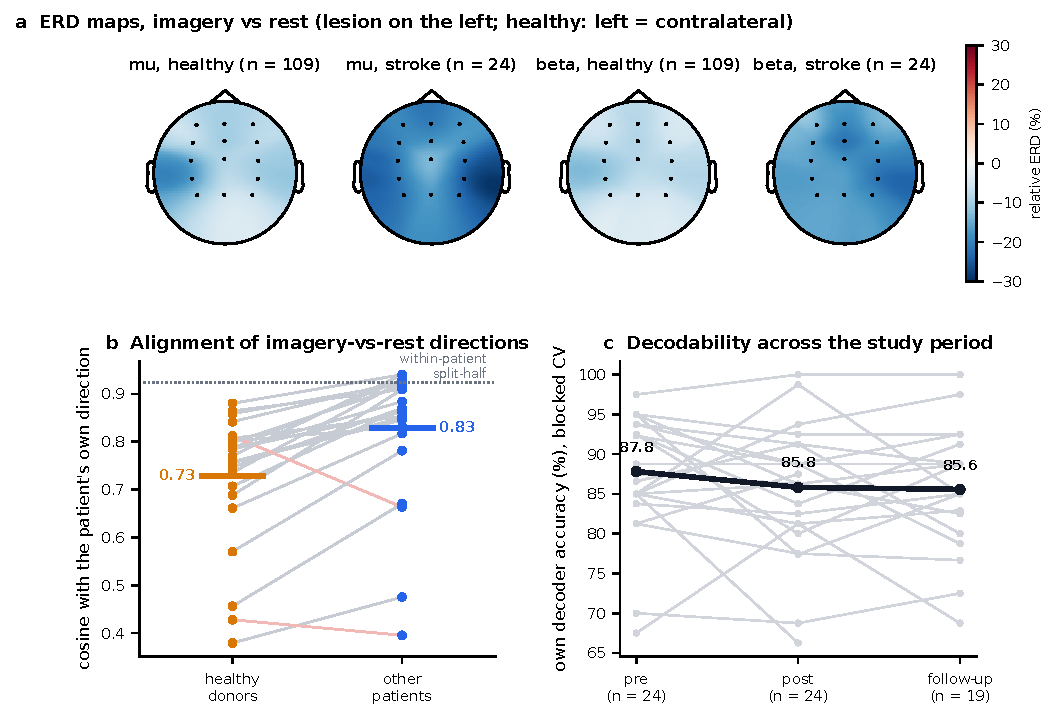
\includegraphics[width=\textwidth]{figures/fig6_neuro.pdf}
\caption{Neurophysiology of S3 and the healthy cohort: (a) ERD maps, (b) decision directions, (c) accuracy across time points.}\label{fig:neuro}
\end{figure}

\subsection{Safety gate and streaming operation}\label{sec:res-gate}

When the transferred decoder was EEGNet pretrained with LesionSim data, always transferring harmed 9 of 16 development patients with five calibration pairs and 11 of 16 with ten, where harmed means at least 2 points below the own decoder. The gate harmed 2 and 1 (exact McNemar tests, $p = 0.008$ and $p = 0.001$), and Figure~\ref{fig:gate}a shows these counts next to those of always averaging the two decoders. It also raised mean accuracy over always transferring, by 4.2 points with five pairs (95\% CI 0.0 to 8.6, $p = 0.032$) and by 8.1 points with ten (1.7 to 13.3, $p = 0.001$; Figure~\ref{fig:gate}b). The gate mostly kept the patient's own decoder and did not beat always using it (80.6\% versus 81.7\%, and 84.4\% versus 84.7\%). Its value is safety: when it is not known whether a transferred model helps a given patient, the gate decides from calibration data alone. With five pairs it abstained for 4 patients, and the remaining 12 reached 83.5\%.

\begin{figure}[!htbp]
\centering
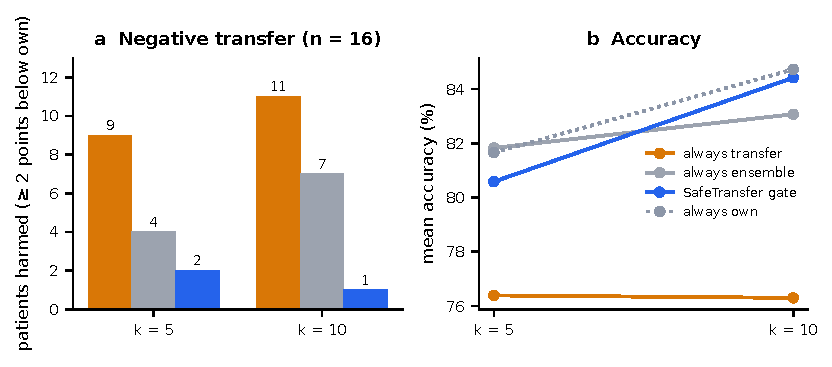
\includegraphics[width=0.78\textwidth]{figures/fig4_safetransfer.pdf}
\caption{SafeTransfer gate (S3): (a) patients harmed and (b) mean accuracy.}\label{fig:gate}
\end{figure}

Streaming each S3 locked test patient's raw recording through the online pipeline gave the same results as the offline evaluation. With five calibration pairs, the own decoder averaged 77.1\% both online and offline, and the pooled decoder 82.5\% online against 81.4\% offline; the differences for individual patients came only from the causal filter. Processing took a median of 12.6\,ms per epoch in this streaming check. Over real LSL streams, with the machine under full load, it took 21 to 23\,ms, with a maximum of 54\,ms, and the final accuracies were identical to the streaming check. A decision is therefore available about 4\,s after each cue, at the end of the imagery window.

\subsection{Negative findings and limitations}\label{sec:res-limits}

This subsection reports in full the results that did not support the decoder or that bound its claims, followed by the evaluation pitfalls and the limitations of the study.

\paragraph{Healthy and generic sources.} On S3 (Figure~\ref{fig:strategies}), every finetuned deep variant trailed the own decoder at both calibration sizes, by 4.5 to 12.2 points. Pretraining on healthy data gave 76.6\% and 76.3\%, adding a LesionSim copy 76.3\% and 76.5\%, adding a copy with generic augmentation 74.5\% and 72.5\%, and adding the other patients 77.2\% and 76.3\%; the deep models barely profited from twice as much calibration data. The frozen CBraMod probe trailed by 14 to 24 points (58.2\% to 68.2\%). Pooling healthy donors into the recentred Riemannian decoder did not help (78.9\% and 84.3\%), and neither did LesionSim donors in population mode (79.7\% and 84.2\%) or in matched mode (78.6\% and 83.5\%).

\paragraph{LesionSim.} Real patients were better donors than healthy participants by 5.1 points (84.0\% versus 78.9\% with five pairs). If LesionSim captured what distinguishes stroke data, its output should have fallen between the two. Figure~\ref{fig:lesionsim} shows that it did not, for any of its learned settings. Each cell is the mean accuracy of the pooled decoder with five calibration pairs and healthy donors transformed by one combination of the attenuation $\alpha$, the contralesional shift $\beta$ and the spread $s$ between trials.
\begin{itemize}
\item All 27 learned settings scored between 78.5\% and 80.0\%.
\item Chosen honestly across patients, the best setting gave 78.8\%, no better than unmodified healthy donors (median $-0.7$ points, $p = 0.86$). It closed none of the gap, and even the best setting in hindsight closed only 21\% of it.
\item The honestly chosen setting differed in every fold.
\item In matched mode, the estimated attenuation and shift mostly sat at their bounds, with $\alpha = 1$ and $\beta = 1$ in the median. The chronic patients' ipsilesional mu desynchronisation was usually not weaker than the healthy participants' ($-13\%$ ipsilateral and $-9\%$ contralateral on average), contrary to the premise of operator O1.
\end{itemize}

\begin{figure}[!htbp]
\centering
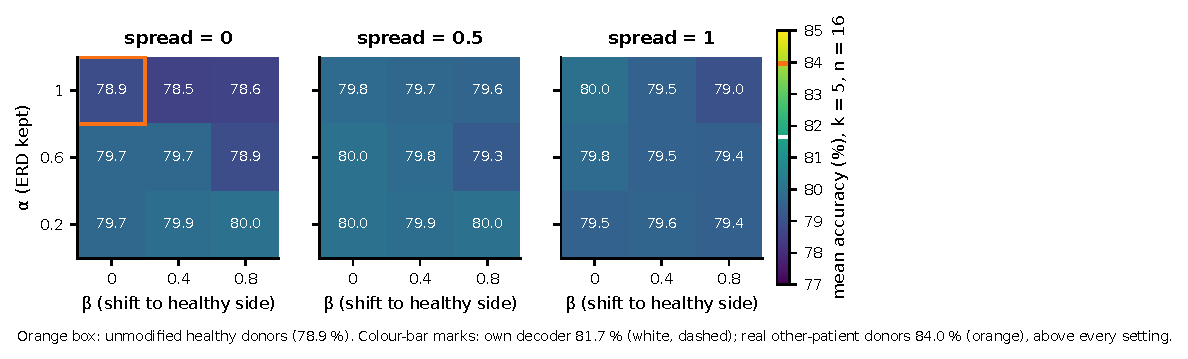
\includegraphics[width=0.86\textwidth]{figures/fig3_lesionsim_settings.pdf}
\caption{LesionSim settings (S3, five calibration pairs).}\label{fig:lesionsim}
\end{figure}

\paragraph{Imagery of the left versus the right hand in acute stroke.} Within patients (blocked cross validation, 34 development patients), the own decoder reached 57.7\%, with 8 patients at or above the chance threshold of 65\%. None of the following beat it: EEGNet trained from scratch (57.4\%) or pretrained on healthy data and finetuned (55.7\%); the frozen foundation model probe (52.1\% to 52.9\%); slow cortical potentials (57.2\%); phase lagged coherence (46.7\% to 52.4\%); individually tuned frequency bands (53.4\%); and eleven variants of the classical decoder (regularisation, discriminant analysis, minimum distance to the mean, common spatial patterns (CSP), channel subsets, time crops and outlier removal). LesionSim did not improve healthy pretraining either (54.5\% to 56.2\% for single operators and their combination, against 56.5\% for healthy data alone). Strikingly, pretraining on the other development patients' real recordings gave no gain (56.0\%).

Figure~\ref{fig:beijing} gathers three analyses on S1: the choice of window and band for each patient in panel a, which the evaluation pitfalls below discuss, the window ensemble in panel b and the gate in panel c. The window ensemble ens16 was the only decoder that improved significantly on the own decoder during development, before correction: 61.5\% versus 57.4\% on the same 39 trials. It helped 20 patients and harmed 9, raised the number of patients above chance from 8 to 13, and gave $p = 0.012$ (0.13 after Holm correction over 11 variants). The gain needed the window after imagery, without which the ensemble scored 58.2\%. On the 15 locked test patients the ensemble improved by a similar amount (+3.6 points), but the preregistered one sided test gave $p = 0.083$ (Table~\ref{tab:prereg}). Figure~\ref{fig:beijing}b shows the ensemble against the base decoder for every development and locked patient, red where accuracy fell.

Whether a patient can use a BCI of the left versus the right hand could be predicted from calibration data but not from clinical scores. Under chronological calibration on the first 20 trials, the gate passed 8 of 34 development patients. These scored 72.6\% on their later trials, against 51.8\% for the 26 it abstained on ($p < 0.001$). Calibration and later accuracy correlated ($\rho = 0.48$, $p = 0.004$), while later accuracy was unrelated to stroke severity (NIHSS, $\rho = -0.05$) or to time since stroke ($\rho = -0.13$). Figure~\ref{fig:beijing}c plots each patient's calibration accuracy on the first 20 trials, from cross validation that leaves out one pair at a time, against the accuracy on the later trials, with the patients passed by the gate in blue. On the locked test patients the gate passed only one patient (78.9\% on later trials), so the preregistered comparison was not evaluable. With a portable system of 29 channels and 40 trials, most patients did not reach significance with any decoder. A short screening session could therefore decide whether feedback driven by imagery is worth offering, and the gate's abstention is the honest output for the rest.

The baselines published with S1 were not reached on its raw data. The analysis code released with the dataset gave 50.56\% (CSP with linear discriminant analysis; 95\% CI 47.8 to 53.4) and 49.29\% (a filter bank of CSP with an SVM; 46.9 to 51.7), against published values of 55.57\% and 57.57\%~\cite{liu2024}. The cleaned recordings gave the same (51.86\% and 49.17\%), in line with the success rates of 49.46\% to 51.82\% that a reinforcement learning decoder reached on this cohort~\cite{via2026}. An audit of the 34 development patients that used no labels explains part of the difficulty:
\begin{itemize}
\item every patient had between 1 and 9 technically faulty channels, and 27 had at least one faulty motor channel;
\item a rhythm peak above the aperiodic background was present in only 20 patients;
\item the classic lateralised power difference between C3 and C4 was significant in only 2 patients in the mu band and 4 in the beta band, against 1.7 expected by chance.
\end{itemize}

\begin{figure}[!htbp]
\centering
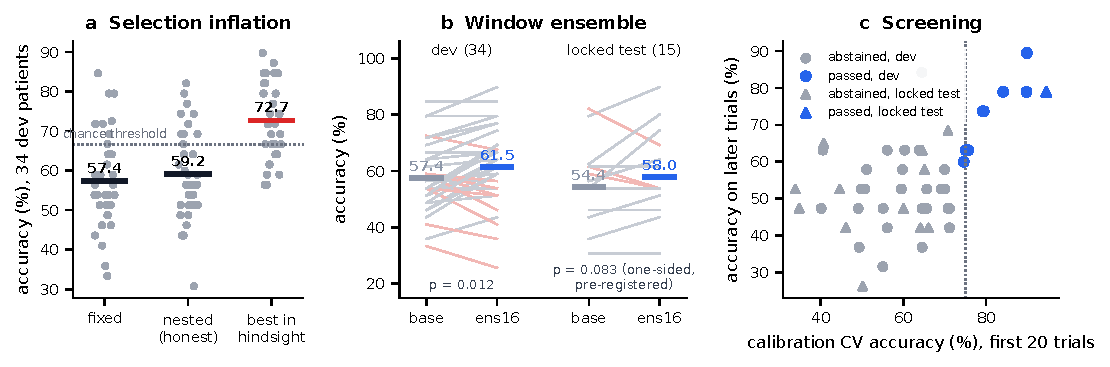
\includegraphics[width=\textwidth]{figures/fig5_beijing.pdf}
\caption{S1, acute stroke: (a) window and band choice, (b) window ensemble, (c) calibration screen.}\label{fig:beijing}
\end{figure}

\paragraph{Combinations that did not help.} An empirical Bayes prior on the decoder weights, used instead of pooling donor trials, was worse than pooling in every setting, and augmentation with subwindows and unsupervised adaptation of the bias did not help. The third declared round tried forgetting old trials, a fixed donor weight, donors from every session, experts on early and late time windows and a larger model average. None beat model averaging by more than 1 point in any cohort or setting, and choices made on one cohort added between 0.0 and 0.9 points on the other. The combination has reached a plateau of about 90\% on S3 and 80\% on S4.

\paragraph{Evaluation pitfalls.} Five pitfalls produced effects as large as the differences between methods, and we report them so that others can avoid them.
\begin{enumerate}
\item \textbf{Tuning each patient without nesting.} Choosing each patient's best window and band in hindsight gave 72.7\% on S1, while the same choice made honestly by nested cross validation gave 59.2\%, against 57.4\% for a fixed choice (Figure~\ref{fig:beijing}a). The gap of 13.5 points is selection luck on 40 trials.
\item \textbf{Transductive drift correction.} Recentring each block of test trials on its own mean improved accuracy by 5.1 points ($p = 0.016$), but the gain vanished when only past trials could be used, as in a real session. It came from looking ahead.
\item \textbf{Euclidean alignment on data referenced to the common average.} A plain inverse square root amplified the null direction of such data by a factor of about $10^6$, which injected noise into every aligned input and pushed edited copies to values near $10^7$. With the plain inverse square root, EEGNet pretrained on healthy data appeared to harm 22 of 34 patients significantly ($p = 0.034$). With the null directions dropped, held out healthy accuracy rose from 63.0\% to 67.7\%, and the apparent negative transfer disappeared (15 helped, 16 harmed, $p = 0.26$).
\item \textbf{Floating point ties in rank tests.} Accuracies are fractions of a few dozen trials, and equal differences, such as four patients each gaining one of 70 test trials, came out of floating point arithmetic a few units in the last place apart. The Wilcoxon test then ranked them apart instead of as ties, which would turn the correct $p = 0.047$ of the S3 locked test into 0.035. All reported $p$ values are computed with differences rounded to $10^{-9}$.
\item \textbf{Updates after every trial in alternating designs.} Coadaptive updating after every trial carried the trial order of S3 into the decoders and changed the margin of the combined decoder over coadaptive recalibration from 3.0 to 5.2 points (Section~\ref{sec:res-audit}).
\end{enumerate}
Locked test sets, chronological calibration, preregistered confirmation run once, and statistics computed from the saved results kept these effects out of the conclusions.

\paragraph{Limitations.} The locked test sets are small, with 8 and 15 patients, and the combined decoder was confirmed at one site; at a second hospital it beat the own decoder but not coadaptive recalibration. All analyses are offline, with no feedback to patients in a closed loop and no clinical outcome, and the largest gains need the cue label of every trial during the session. Decoding of imagery versus rest partly reflects engagement outside the motor system, and the healthy donors were recorded on different devices from the patients, so part of the gap between healthy and stroke donors may be technical.

\section{Conclusion}\label{sec:conclusion}

For motor imagery BCIs after stroke, data from other stroke patients and from the patient's own earlier sessions shorten calibration. Pooling other patients raised accuracy on locked test patients from 77.1\% to 81.4\% with five calibration pairs, more than the patient's own decoder reached with ten, and the gain held on a second cohort. There, a bank of mu, low beta and high beta covariances added 2.3 points, and a returning patient's earlier sessions added 3.2 points and, without any new labels, did not fall below five labelled calibration pairs. A gate that uses only calibration data cut the number of patients harmed by transfer from 9 to 2. Combined with online recentring, coadaptive updating and online model averaging, these sources raised accuracy on held out patients from 77.1\% to 88.7\% in the first session and from 75.9\% to 88.1\% in later sessions, every patient improved, and the decoder exceeded coadaptive recalibration of the patient's own decoder by 3.0 points. Returning patients gained 11.9 points with no labels after calibration and 8.4 points with no labels at all, and every confirmed gain survived the audits for leakage. At a second hospital, on a weaker task, the decoder added 4.4 points over the patient's own decoder, although not significantly more than coadaptive recalibration. Building such systems will depend on shared, harmonised patient data and on keeping each patient's history.

\backmatter

\bibliography{references}

\section*{Declarations}

\begin{itemize}
\item \textbf{Supplementary information} \; Not applicable.
\item \textbf{Acknowledgements} \; Not applicable.
\item \textbf{Funding} \; No funding was received for this research.
\item \textbf{Conflict of interest/Competing interests} \; The authors declare that they have no competing interests.
\item \textbf{Ethics approval} \; Not applicable. The study is a secondary analysis of publicly available EEG datasets released by their original investigators, and no new data were collected from human participants.
\item \textbf{Consent to participate} \; Not applicable.
\item \textbf{Consent for publication} \; All authors consent to the publication of this manuscript.
\item \textbf{Availability of data, materials and code} \; The study uses the public recordings of S1~\cite{liu2024}, S3~\cite{wang2026} and S4~\cite{liu2025gait} and the PhysioNet motor movement and imagery database~\cite{schalk2004,goldberger2000}, each read from its original release. The code that builds the harmonised benchmark, every experiment script, the tables of results for each patient that support every number in this article, the scripts that generate every table and figure, the streaming implementation and the preregistration log with its commit history are available at \url{https://github.com/prayag-1771/HemiShift}.
\item \textbf{Authors' contributions} \; Prayag Sharma conceived the study, designed and implemented the experiments, performed the statistical analysis, produced all figures and tables, and drafted the manuscript. Ravi Tiwari supervised the work and reviewed the manuscript. All authors read and approved the final version of the manuscript.
\end{itemize}

\end{document}
